\chapter{MATERIAL E MÉTODO}
\label{chap:metodologia}

Este capítulo descreve a abordagem adotada para o desenvolvimento da ferramenta
de apoio à gestão de equipamentos médico-hospitalares e o método de tratamento
dos dados que sustenta os resultados apresentados no capítulo seguinte. Trata-se
de uma pesquisa aplicada, de natureza quantitativa e caráter exploratório,
conduzida na forma de desenvolvimento de software seguido de um estudo de caso
com dados reais do parque de equipamentos do HC-UFPE.

\section{Tecnologias e arquitetura da ferramenta}

A ferramenta foi implementada como uma aplicação \textit{desktop} em linguagem
Python (versão 3.12)~\cite{python312}, estruturada segundo o paradigma ETL. A
interface gráfica foi construída com a biblioteca PySide6 (\textit{bindings}
oficiais do \textit{framework} Qt 6)~\cite{pyside6}, enquanto a manipulação e o
tratamento dos dados utilizam a biblioteca pandas~\cite{pandas}. O gerenciamento
de dependências e o empacotamento do projeto são feitos com o
Poetry~\cite{poetry}, e a distribuição para o ambiente hospitalar (Windows) é
gerada como executável único por meio do PyInstaller~\cite{pyinstaller}.

A aplicação organiza-se em duas camadas principais: (i) uma camada de
transformação de dados, responsável por extrair, normalizar e cruzar as planilhas
de origem; e (ii) uma camada de apresentação, que calcula os indicadores e os
exibe em um painel interativo dividido em uma aba de Análise (gráficos e
indicadores) e uma aba de Dados (tabelas consultáveis). A separação entre
transformação e apresentação permite que a mesma base tratada alimente diferentes
visualizações de forma consistente. A \ref{fig:aba_dados} ilustra a aba de
Dados, na qual a base consolidada pode ser consultada em formato tabular.

\begin{figure}[H]
    \centering
    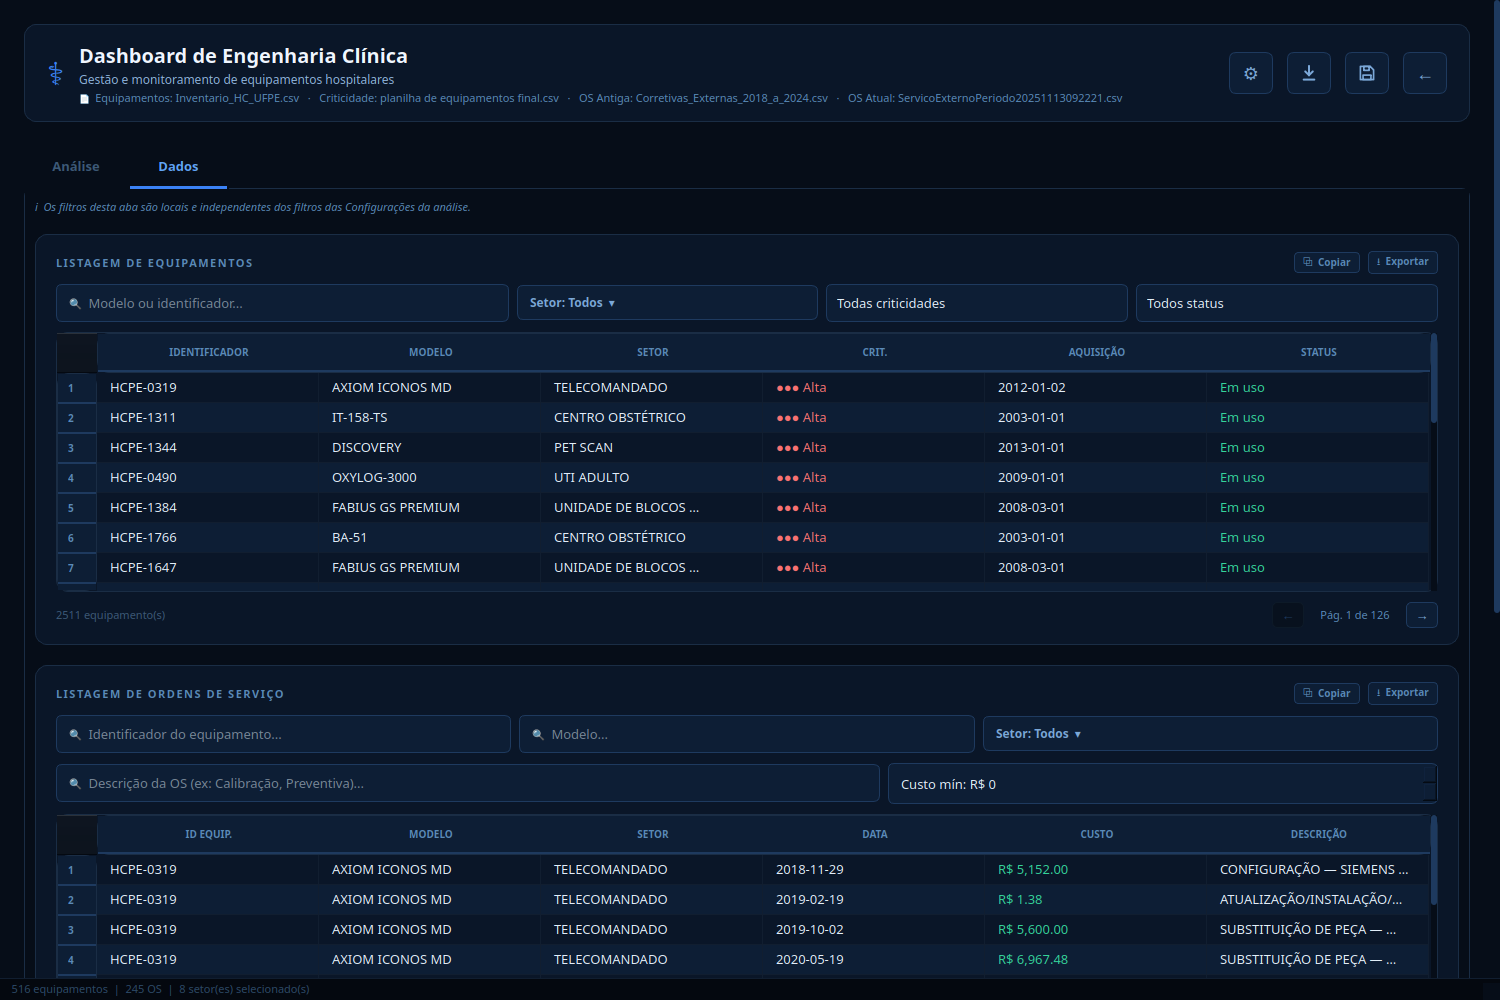
\includegraphics[width=\textwidth]{./imagens/04_aba_dados.png}
    \captionsource{fig:aba_dados}{Aba de Dados da ferramenta, com a base consolidada em formato tabular}{Elaborado pelo autor (2026)}
\end{figure}

\section{Fontes de dados}
\label{sec:fontes}

Foram utilizados quatro arquivos no formato CSV, fornecidos pela engenharia
clínica do HC-UFPE, organizados em quatro papéis distintos, conforme a
\ref{tab:fontes}.

\begin{table}[H]
    \centering
    \begin{tabular}{lp{9cm}}
        \hline
        \textbf{Insumo} & \textbf{Conteúdo} \\
        \hline
        Inventário & Cadastro dos equipamentos: identificador, modelo, localização (setor), data de aquisição e valor. \\
        Criticidade & Peso de criticidade por modelo de equipamento (escala de 1 a 3). \\
        OS --- formato antigo & Ordens de serviço corretivas no padrão legado, com datas e valores em convenção brasileira. \\
        OS --- formato atual & Ordens de serviço corretivas no padrão recente, com datas em formato ISO e valores em convenção norte-americana. \\
        \hline
    \end{tabular}
    \captionsource{tab:fontes}{Fontes de dados utilizadas e seus papéis}{Elaborado pelo autor (2026)}
\end{table}

A coexistência de dois formatos distintos de ordens de serviço --- resultado de
uma mudança no sistema de registro ao longo do tempo --- constitui um dos
principais desafios de integração tratados pela ferramenta, uma vez que cada
formato adota convenções diferentes de nomes de colunas, de representação de
datas e de separadores numéricos.

No estudo de caso conduzido neste trabalho, esses quatro papéis foram preenchidos
pelos arquivos reais do HC-UFPE listados na \ref{tab:arquivos}.

\begin{table}[H]
    \centering
    \begin{tabular}{ll}
        \hline
        \textbf{Insumo} & \textbf{Arquivo} \\
        \hline
        Inventário de equipamentos & \texttt{Inventario\_HC\_UFPE.csv} \\
        Criticidade & \texttt{planilha de equipamentos final.csv} \\
        OS --- formato antigo & \texttt{Corretivas\_Externas\_2018\_a\_2024.csv} \\
        OS --- formato atual & \texttt{ServicoExternoPeriodo20251113092221.csv} \\
        \hline
    \end{tabular}
    \captionsource{tab:arquivos}{Arquivos utilizados no estudo de caso do HC-UFPE}{Elaborado pelo autor (2026)}
\end{table}

\section{Processo de tratamento dos dados (ETL)}

\subsection*{Extração}

Cada arquivo CSV é lido tendo o ponto e vírgula como separador de campos. O
formato antigo de OS exige o descarte da primeira linha (cabeçalho duplicado), e
a planilha de criticidade possui o cabeçalho útil a partir da sexta linha, da
qual se aproveitam apenas as colunas de modelo e peso de criticidade.

\subsection*{Transformação e normalização}

A etapa central do processo é a unificação dos dois formatos de OS em um esquema
canônico único. Antes da concatenação, os valores são normalizados de acordo com
a sua origem, evitando ambiguidades de interpretação, conforme a
\ref{tab:normalizacao}.

\begin{table}[H]
    \centering
    \begin{tabular}{p{2.8cm}p{5cm}p{5cm}}
        \hline
        \textbf{Atributo} & \textbf{Formato antigo (BR)} & \textbf{Formato atual (ISO/US)} \\
        \hline
        Datas & dd/mm/aaaa (dia primeiro) & aaaa-mm-dd (ISO, sem ambiguidade) \\
        Valores monetários & ponto = milhar; vírgula = decimal & ponto = decimal \\
        Descrição do serviço & tipo de serviço + assistência & fornecedor \\
        \hline
    \end{tabular}
    \captionsource{tab:normalizacao}{Normalização dos atributos por formato de origem}{Elaborado pelo autor (2026)}
\end{table}

Em seguida, os nomes das colunas de ambos os formatos são mapeados para um
conjunto canônico (ordem de serviço, equipamento, data de abertura, data de
fechamento, serviço/assistência e identificador), e os registros são concatenados
em uma única base de ordens de serviço.

\subsection*{Carga e cruzamento (integração)}

A base unificada de OS é então cruzada com o inventário. Como as ordens de
serviço armazenam o identificador no padrão ``TAG,Patrimônio'' enquanto o
inventário utiliza apenas a TAG, ambos os lados são normalizados para a TAG
(porção anterior à primeira vírgula) antes do casamento --- procedimento que
evita a perda de uma parcela expressiva dos vínculos. Registros de OS sem
identificador são descartados para não corromper o custo atribuído aos demais
equipamentos. A criticidade é incorporada por meio da junção da planilha de pesos
com o inventário pelo nome do modelo; modelos sem correspondência recebem
criticidade mínima (nível 1). O custo de cada ordem de serviço é agregado por
equipamento, produzindo o custo total de manutenção corretiva de cada item. Ao
final, cada equipamento é representado por uma estrutura que reúne modelo, setor,
criticidade, data de aquisição, valor, custo acumulado e a lista de ordens de
serviço associadas, pronta para alimentar os indicadores do painel.

\section{Índice de priorização e modelo de otimização multicritério}
\label{sec:score}

Para apoiar a decisão de substituição, a ferramenta calcula um índice de
prioridade (\textit{score}) na escala de 0 a 100, combinando três critérios
complementares, conforme a \ref{tab:score}.

\begin{table}[H]
    \centering
    \begin{tabular}{lp{7cm}r}
        \hline
        \textbf{Critério} & \textbf{Regra} & \textbf{Pontuação máxima} \\
        \hline
        Idade & Equipamentos com 10 anos ou mais recebem a pontuação cheia & 20 pontos \\
        Criticidade & Proporcional ao nível de criticidade (nível $\div$ 3 $\times$ 50) & 50 pontos \\
        Custo de manutenção & Proporcional ao custo acumulado em relação ao maior custo do parque & 30 pontos \\
        \hline
    \end{tabular}
    \captionsource{tab:score}{Critérios e pontuações do índice de priorização}{Elaborado pelo autor (2026)}
\end{table}

A escolha desses três critérios --- criticidade, idade e custo de manutenção ---
alinha-se aos fatores recorrentemente adotados na literatura de priorização de
substituição de equipamentos médico-hospitalares~\cite{park2025evaluation,zamzam2021prioritisation}.
A pontuação de custo emprega uma normalização do tipo min-max, escalonando o custo
acumulado de cada item em relação ao maior custo do parque~\cite{sinsomboonthong2022performance}.

A criticidade é o critério de maior peso, refletindo a prioridade clínica do
equipamento; a idade e o custo histórico de manutenção complementam a avaliação,
capturando, respectivamente, o envelhecimento e o ônus financeiro acumulado. O
painel permite ajustar interativamente tanto os pesos de cada critério quanto o
limite de idade considerado, recalculando o ranking em tempo real --- o que
confere à ferramenta um caráter exploratório e adaptável a diferentes políticas
de gestão.

A partir desse índice, a ferramenta materializa um modelo de otimização
multicritério para a alocação do orçamento de substituição. Dado um orçamento
disponível, informado pelo gestor, a funcionalidade de distribuição de orçamento
percorre os equipamentos em ordem decrescente de prioridade e seleciona aqueles
cuja substituição cabe no recurso disponível, de modo a maximizar o impacto
agregado em segurança e em redução de custo. Dessa forma, o \textit{score} deixa
de ser apenas um ranking e passa a orientar objetivamente \textit{quais}
equipamentos substituir diante de uma restrição orçamentária --- traduzindo a
priorização multicritério em uma recomendação de alocação de recursos.

\section{Recorte de análise e indicadores gerados}

Por padrão, a ferramenta aplica um recorte sobre os setores de maior criticidade
assistencial (UTI Adulto, UTI Neonatal, Bloco Cirúrgico e Centro Obstétrico),
seleção que pode ser ampliada ou alterada pelo usuário no menu de configurações.
Sobre o conjunto filtrado, são calculados os seguintes indicadores: total de
equipamentos, total de ordens de serviço e gasto total (KPIs); distribuição
etária do parque; ranking de prioridade de substituição; histórico mensal e anual
de emissão de OS; evolução do custo por ano; custo por setor; e os equipamentos
de maior custo acumulado. Todos os indicadores reagem dinamicamente aos filtros
aplicados.

\section{Procedimento de execução e validação}

O fluxo de uso parte de uma tela de importação, na qual o usuário seleciona as
quatro planilhas. Após o processamento --- executado em segundo plano para
preservar a responsividade da interface --- é exibida uma pré-visualização da
base de OS consolidada para conferência antes da confirmação. Confirmada, a
aplicação apresenta o painel de análise. As seleções de arquivos e as
configurações de análise podem ser salvas e recarregadas, garantindo a
reprodutibilidade dos estudos. Os resultados reportados no capítulo seguinte foram
obtidos exatamente por esse procedimento, carregando-se as quatro planilhas reais
do HC-UFPE e processando-as com a ferramenta.
